\documentclass[aps,prd,longbibliography,reprint,twocolumn,amsmath,amssymb,amsfonts,showpacs,superscriptaddress]{revtex4-1}%reprint

\linespread{1.2}



\usepackage{graphicx, epsfig, amssymb}
\usepackage{amsmath, amsfonts}
\usepackage{bm}
\usepackage{enumitem}
\usepackage[usenames]{color}
\definecolor{navyblue}{rgb}{0.0, 0.0, 0.5}
\usepackage{hyperref}
\hypersetup
	{
		colorlinks,%
		citecolor=blue,%
		linkcolor=red,%
		urlcolor=blue,%
	}


%\usepackage[linktocpage,colorlinks=true,linkcolor=red]{hyperref}
\usepackage[caption=false]{subfig}
\usepackage[utf8]{inputenc}
\usepackage{tensor}
\usepackage{soul}
%\usepackage{enumerate}
\usepackage{pict2e}
\usepackage{diagbox}
\usepackage{empheq}

%\usepackage[margin=1in]{geometry}
\usepackage{float}
%\usepackage{subfig}
\usepackage{comment}
\usepackage{array}
%\usepackage{varioref}
%\usepackage[hidelinks]{hyperref}
%\usepackage{cleveref}
%\usepackage[numbers]{natbib}
\usepackage{units}
\usepackage{wasysym}
%\usepackage{caption}
%\usepackage{subcaption}



\DeclareMathAlphabet{\mathpzc}{OT1}{pzc}{m}{it}
\newcommand{\ff}{\hat{f}}

\def\l{\left}
\def\r{\right}
\def\p{\partial}

\newcommand{\angarg}{(\theta,\phi)}
\newcommand{\dth}{\frac{d}{d \theta}}
\newcommand{\sh}{ {}_{-s} S_{\ell m}^{a \omega}}
\newcommand{\zh}{ {}_{-s} Z_{\ell m}^{a \omega}}
\newcommand{\syjm}{  {}_{-s}Y_{jm} }
\newcommand{\sylm}{  {}_{-s} Y_{\ell m} }
\newcommand{\sumjm}{\sum_{j=s}^{\infty} \sum_{m=-j}^{j}}
\newcommand{\sumjms}{\sum_{j,m}}
\newcommand{\cS}{\mathcal{S}}
\newcommand{\lmws}{{\ell m \omega s}}
\newcommand{\nn}{\nonumber}

\newcommand*\widefbox[1]{\fbox{\rule[-2cm]{0pt}{4cm}\hspace{2em}#1\hspace{2em}}}

\newcommand{\sam}[1]{\textcolor{red}{(Sam: #1)}}
\newcommand{\tom}[1]{\textcolor{blue}{(Tom: #1)}}
\newcommand{\mo}[1]{\textcolor{green}{(Mohamed: #1)}}

\renewcommand{\arraystretch}{1.3} % espace entre les lignes de la table
%\setlength{\tabcolsep}{.3cm} % espace entre les colonnes de la table

\usepackage{footnote}
\usepackage{tablefootnote}


\usepackage{threeparttable}


\begin{document}

\title{Scattering from compact objects, Regge poles \\ and the Complex Angular Momentum method}



\author{Mohamed \surname{Ould~El~Hadj}}
\email{m.ouldelhadj@sheffield.ac.uk}

\affiliation{Equipe Physique
Th\'eorique, SPE, UMR 6134 du CNRS
et de l'Universit\'e de Corse,\\
Universit\'e de Corse, Facult\'e des Sciences, BP 52, F-20250 Corte,
France}

\affiliation{Consortium for Fundamental Physics,  School of Mathematics and Statistics,
University of Sheffield, Hicks Building, Hounsfield Road, Sheffield S3 7RH, United Kingdom \looseness=-1}
%
\author{Tom Stratton}\email{tstratton1@sheffield.ac.uk}
\affiliation{Consortium for Fundamental Physics,  School of Mathematics and Statistics,
University of Sheffield, Hicks Building, Hounsfield Road, Sheffield S3 7RH, United Kingdom \looseness=-1}
%
\author{Sam R. Dolan}\email{s.dolan@sheffield.ac.uk}
\affiliation{Consortium for Fundamental Physics,  School of Mathematics and Statistics,
University of Sheffield, Hicks Building, Hounsfield Road, Sheffield S3 7RH, United Kingdom \looseness=-1}
%
\begin{abstract}
To be written
\end{abstract}

\date{\today}

\maketitle

\tableofcontents

\section{Introduction}


 The topic of time-independent scattering by compact bodies in the gravitational context has been studied in detail since the 1960s \cite{Hildreth1964PhDT64, Matzner:1968, Vishveshwara:1970}, and there now exists a substantial literature exploring the scattering of scalar, spinor, electromagnetic and gravitational waves \cite{Mashhoon:1973zz,Chrzanowski:1976jb,DeLogi:1977dp,Sanchez:1977vz,MatznerRyan1978,Handler:1980un,Matzner:1985rjn,Futterman:1988ni,Andersson:1995vi,Glampedakis:2001cx,Dolan:2006vj,Dolan:2007ut,Dolan:2008kf,Crispino:2009xt,Cotaescu:2014jca,Sorge:2015yoa,Gussmann:2016mkp,Leite:2017zyb,Nambu:2019sqn, Folacci:2019vtt,Leite:2019eis}.



\section{Differential scattering cross sections for scalar waves, their CAM representation and their Regge pole approximations}
\label{SecII}


In this section we describe the model for our compact object. Then we recall the partial wave expansions of the differential scattering cross section for plane monochromatic scalar waves impinging upon a compact body. Finally we apply the CAM-approach developed for black-hole scattering in \cite{Folacci:2019cmc} and \cite{Folacci:2019vtt}.

\subsection{Our model}
\label{SecIIa}

  We consider that the gravitating source is a spherically symmetric incompressible perfect fluid ball of uniform
density (see Ref~\cite{Dolan:2017rtj} and references therein). In a coordinate system $\{t,r,\theta,\varphi\}$, the object is described by the metric
\begin{equation}\label{Line_elem}
  ds^2= -f(r) dt^2+h(r)^{-1}dr^2+r^2d\sigma_2^2
\end{equation}
where $d\sigma_2^2$ denotes the metric on the unit 2-sphere $S^2$. Here, the radial function $h(r)$ is continuous but not differentiable across the surface of the star $r=R$ and the function $f(r)$ is one, but not twice, differentiable. We recall that, in the exterior of the star (i.e., $r>R$), we have $f(r)=h(r)=a-2M/r$ by Birkhoff's theorem~\cite{VojeJohansen:2005nd}. In the interior of the star (i.e. $r<R$), we use the Schwarzschild solution for an incompressible fluid~\cite{Shapiro1983}

\begin{subequations}\label{Interior_Solution}
\begin{align}\label{Interior_Solution_f}
    f(r) =\frac{1}{4}\left(1-\frac{2 M r^2}{R^3}\right)+\frac{9}{4}\left(1-\frac{2M}{R}\right) \nonumber\\ -\frac{3}{2}
                \sqrt{\left(1-\frac{2M}{R}\right)\left(1-\frac{2 M r^2}{R^3}\right)},
\end{align}
\begin{equation}\label{Interior_Solution_h}
 h(r) =1-\frac{2 M r^2}{R^3}
\end{equation}
\end{subequations}


\subsection{Partial wave expansions of differential scattering cross sections}
\label{SecIIb}

We recall that, for the scalar field, the differential scattering cross section is given by (see, e.g.,\cite{Dolan:2017rtj} and references therein)
\begin{equation}\label{Scalar_Scattering_diff}
  \frac{d\sigma}{d\Omega} = |\hat{f}(\omega,\theta)|^2
\end{equation}
where
\begin{equation}\label{Scalar_Scattering_amp}
 \hat{f}(\omega,\theta) = \frac{1}{2 i \omega} \sum_{\ell = 0}^{\infty} (2\ell+1)[S_{\ell}(\omega)-1]P_{\ell}(\cos\theta)
\end{equation}
denotes the scattering amplitude.  In Eq.~(\ref{Scalar_Scattering_amp}), the functions $P_{\ell}(\cos\theta)$ are the Legendre polynomials \cite{AS65}.  We also recall that the $S$-matrix elements $S_{\ell}(\omega)$ appearing in Eq.~(\ref{Scalar_Scattering_amp}) can be defined from the modes $\phi_{\omega \ell}$ that solve the homogenous radial equation
\begin{equation}
\label{H_Radial_equation}
\left[\frac{d^{2}}{dr_{\ast}^{2}}+\omega^{2}-V_{\ell}(r)\right]\phi_{\omega\ell}= 0,
\end{equation}
where $r^\ast$ denotes the tortoise coordinate defined by  $dr/dr^\ast =\sqrt{f(r)h(r)}$, and
\begin{equation}\label{Inside_Potentiel}
  V_{\ell}(r) =f(r)\left[\frac{\ell(\ell+1)}{r^2}+\frac{h(r)}{2r}\left(\frac{f'(r)}{f(r)}+\frac{h'(r)}{h(r)}\right)\right]
\end{equation}
is the effective potential. Outside the star ($r>R$), $V_{\ell}(r)$ reduces to the Regge-Wheeler potential
\begin{equation}\label{RW_Potentiel}
  V_{\ell}(r) =\left(1-\frac{2M}{r}\right)\left(\frac{\ell(\ell+1)}{r^2}+\frac{2M}{r^3}\right)
\end{equation}
and the tortoise coordinates $r^\ast$ reduces to $r^\ast = r+ 2M \ln [r/(2M) -1]+\mathrm{const}$.

It is important to recall that the modes $\phi_{\omega \ell}$ should have a regular behaviour at the origin $r \to 0$
\begin{equation}\label{bc_1_in}
\phi_{\omega  \ell}(r) \scriptstyle{\underset{r \to 0}{\sim}}
\displaystyle{r^{\ell+1}}.
\end{equation}
The asymptotic behaviour of the modes at spatial infinity $r \to +\infty$ (i.e., for $r_\ast \to +\infty$) is
\begin{equation}\label{bc_2_in}
\phi_{\omega  \ell}(r) \scriptstyle{\underset{r_\ast \to +\infty}{\sim}}
\displaystyle{ A^{(-)}_\ell (\omega) e^{-i\omega r_\ast} + A^{(+)}_\ell (\omega) e^{+i\omega r_\ast}}.
\end{equation}
In this last equation, the coefficients $A^{(-)}_\ell (\omega)$ and  $A^{(+)}_\ell (\omega)$ are complex amplitudes and we have
\begin{equation}\label{Matrix_S}
  S_{\ell}(\omega) =  e^{i(\ell+1)\pi} \, \frac{A_{\ell}^{(+)}(\omega)}{A_{\ell}^{(-)}(\omega)}.
\end{equation}

\subsection{CAM representation of the scattering amplitude}
\label{SecIIc}

To construct the CAM representation, we follow the steps in section~II of the Ref~\cite{Folacci:2019cmc} and recall the main results.


By using the Sommerfeld-Watson transformation \cite{Watson18,Sommerfeld49,Newton:1982qc} which permits us to write
\begin{equation}\label{SWT_gen}
\sum_{\ell=0}^{+\infty} (-1)^\ell F(\ell)= \frac{i}{2} \int_{\cal C} d\lambda \, \frac{F(\lambda -1/2)}{\cos (\pi \lambda)}
\end{equation}
with a function $F$ without any singularities on the real $\lambda$ axis, we replace the discrete sum over the ordinary angular momentum $\ell$ in Eq.~(\ref{Scalar_Scattering_amp}) by a contour integral in the complex $\lambda$ plane (i.e., in the complex $\ell$ plane with $\lambda = \ell +1/2$). By noting that $P_\ell (\cos \theta)=(-1)^\ell P_\ell (-\cos \theta)$, we obtain
\begin{eqnarray}\label{SW_Scalar_Scattering_amp}
& & \hat{f}(\omega,\theta) = \frac{1}{2 \omega}  \int_{\cal C} d\lambda \, \frac{\lambda}{\cos (\pi \lambda)} \nonumber \\
&&  \qquad\qquad   \times \left[ S_{\lambda -1/2} (\omega) -1 \right]P_{\lambda -1/2} (-\cos \theta).
\end{eqnarray}
In Eqs.~(\ref{SWT_gen}) and (\ref{SW_Scalar_Scattering_amp}), the integration contour encircles counterclockwise the positive real axis of the complex $\lambda$ plane, i.e., we take ${\cal C}=]+\infty +i\epsilon,+i\epsilon] \cup
[+i\epsilon,-i\epsilon] \cup [-i\epsilon, +\infty -i\epsilon[$ with $\epsilon \to 0_+$ (see Fig.1 Ref~\cite{Folacci:2019cmc}).

The Legendre function of the first kind $P_{\lambda -1/2} (z)$ denotes the analytic extension of the Legendre polynomials $P_\ell (z)$. It is defined in terms of hypergeometric functions by \cite{AS65}
\begin{equation}\label{Def_ext_LegendreP}
P_{\lambda -1/2} (z) = F[1/2-\lambda,1/2+\lambda;1;(1-z)/2].
\end{equation}
In Eq.~(\ref{SW_Scalar_Scattering_amp}), $S_{\lambda -1/2} (\omega)$ denotes ``the'' analytic extension of $S_\ell (\omega)$. It is given by [see Eq.~(\ref{Matrix_S})]
\begin{equation}\label{Matrix_S_CAM}
  S_{\lambda -1/2}(\omega) =  e^{i(\lambda + 1/2)\pi} \, \frac{A_{\lambda -1/2}^{(+)}(\omega)}{A_{\lambda -1/2}^{(-)}(\omega)}
\end{equation}
where the complex amplitudes $A^{(-)}_{\lambda -1/2} (\omega)$ and  $A^{(+)}_{\lambda -1/2} (\omega)$ are defined from the analytic extension of the modes $\phi_{\omega \ell}$, i.e., from the function $\phi_{\omega ,\lambda -1/2}$.

It is important to note that the poles of  $S_{\lambda -1/2} (\omega)$ in the complex $\lambda$ plan (i.e., the Regge poles) are defined  as  the zeros $\lambda_n(\omega)$ with $n=1,2,3,\ldots$ of the coefficient  $A^{(-)}_{\lambda-1/2} (\omega)$ [see Eq.~(\ref{Matrix_S_CAM})]
\begin{equation}\label{PR_def_Am}
A^{(-)}_{\lambda_n(\omega)-1/2} (\omega)=0.
\end{equation}
The residue of the matrix $S_{\lambda-1/2}(\omega)$ at the pole $\lambda=\lambda_n(\omega)$ is defined by [see Eq.~(\ref{Matrix_S_CAM})]
\begin{equation}\label{residues_RP}
r_n(\omega)=e^{i\pi [\lambda_n(\omega)+1/2]} \left[ \frac{A_{\lambda -1/2}^{(+)}(\omega)}{\frac{d}{d \lambda}A_{\lambda -1/2}^{(-)}(\omega)}\right]_{\lambda=\lambda_n(\omega)}.
\end{equation}
These residues play a central role in the complex angular momentum paradigm.


Now, we ``deform'' the contour ${\cal C}$ in Eq.~(\ref{SW_Scalar_Scattering_amp}) in order to collect, by using Cauchy's theorem, the Regge poles contributions. This is achieved by following, \textit{mutatis mutandis}, the approach developed in Ref~\cite{Folacci:2019cmc} (see more particularly Sec. IIB~3 and Fig.~1). We obtain

\begin{equation}\label{CAM_Scalar_Scattering_amp_tot}
\hat{f} (\omega, \theta) =  \hat{f}^\text{\tiny{B}} (\omega, \theta) +  \hat{f}^\text{\tiny{RP}} (\omega, \theta)
\end{equation}
where
\begin{subequations}\label{CAM_Scalar_Scattering_amp_decomp}
\begin{equation}\label{CAM_Scalar_Scattering_amp_decomp_Background}
\hat{f}^\text{\tiny{B}} (\omega, \theta) = \hat{f}^\text{\tiny{B},\tiny{Re}} (\omega, \theta)+ \hat{f}^\text{\tiny{B},\tiny{Im}} (\omega, \theta)
\end{equation}
is a background integral contribution with
\begin{equation}\label{CAM_Scalar_Scattering_amp_decomp_Background_a}
\hat{f}^\text{\tiny{B},\tiny{Re}} (\omega, \theta) = \frac{1}{\pi \omega} \int_{{\cal C}_{-}} d\lambda \, \lambda S_{\lambda -1/2}(\omega) Q_{\lambda -1/2}(\cos \theta +i0)
\end{equation}
and
\begin{eqnarray}\label{CAM_Scalar_Scattering_amp_decomp_Background_b}
\hat{f}^\text{\tiny{B},\tiny{Im}} && (\omega, \theta) = \frac{1}{2 \omega}\left(\int_{+i\infty}^{0} d\lambda \, \left[S_{\lambda -1/2}(\omega) P_{\lambda_n(\omega) -1/2} (-\cos \theta) \right. \right.\nonumber \\
&& -\left. \left. S_{-\lambda -1/2}(\omega) e^{i \pi \left(\lambda+1/2\right)}P_{\lambda_n(\omega) -1/2} (\cos \theta) \right]\lambda\right).
\end{eqnarray}
\end{subequations}
The second term in Eq.~(\ref{CAM_Scalar_Scattering_amp_tot}) ,
\begin{eqnarray}\label{CAM_Scalar_Scattering_amp_decomp_RP}
& & \hat{f}^\text{\tiny{RP}} (\omega, \theta) = -\frac{i \pi}{\omega}    \sum_{n=1}^{+\infty}   \frac{ \lambda_n(\omega) r_n(\omega)}{\cos[\pi \lambda_n(\omega)]}  \nonumber \\
&&  \qquad\qquad \qquad\qquad \times  P_{\lambda_n(\omega) -1/2} (-\cos \theta),
\end{eqnarray}
is a sum over the Regge poles lying in the first quadrant of the CAM plane. Of course, Eqs.~(\ref{CAM_Scalar_Scattering_amp_tot}), (\ref{CAM_Scalar_Scattering_amp_decomp}) and (\ref{CAM_Scalar_Scattering_amp_decomp_RP}) provide an exact representation of the scattering amplitude $\hat{f} (\omega, \theta)$ for the scalar field, equivalent to the initial partial wave expansion (\ref{Scalar_Scattering_amp}). From this CAM representation, we can extract the contribution $\hat{f}^\text{\tiny{RP}} (\omega, \theta)$ given by (\ref{CAM_Scalar_Scattering_amp_decomp_RP}) which, as a sum over Regge poles, is only an approximation of $\hat{f} (\omega, \theta)$, and which provides us with an approximation of the differential scattering cross section (\ref{Scalar_Scattering_diff}).

\section{Reconstruction of differential scattering cross sections from Regge pole sums}
\label{SecIII}

In this section,  we compare the partial wave expansions of the differential scattering cross sections with their equivalent CAM representations or, more precisely, their Regge pole approximations.

\subsection{Computational methods}
\label{SecIIIa}

To construct the scattering amplitude \eqref{Scalar_Scattering_amp}, the back ground integrals~\eqref{CAM_Scalar_Scattering_amp_decomp_Background_a} and~\eqref{CAM_Scalar_Scattering_amp_decomp_Background_b} as well as the Regge pole contribution~\eqref{CAM_Scalar_Scattering_amp_decomp_RP}, we use, \textit{mutatis mutandis} the computational methods that permitted one of us, in Refs~\cite{Folacci:2019cmc,Folacci:2019vtt} to consider the CAM representation for scattering of the scalar, electromagnetic and gravitational waves by Schwarzschild BH (see also Ref~\cite{Dolan:2017rtj}). It is important to remark that, duo to the long rang nature of the field propagating on the Schwarzschild BH (outside the compact body), the scattering amplitude~\eqref{Scalar_Scattering_amp} and the background integral~\eqref{CAM_Scalar_Scattering_amp_decomp_Background_a} suffer a lack of convergence and to overcome this problem, i.e., to accelerate the convergence of this sum and integral, we have used the method described in the Appendix of Ref~\cite{Folacci:2019cmc}. We have performed all the numerical calculations by using {\it Mathematica} \cite{Mathematica}.


\subsection{Results and comments}
\label{SecIIIb}




 \begin{figure}[htb]
\centering
 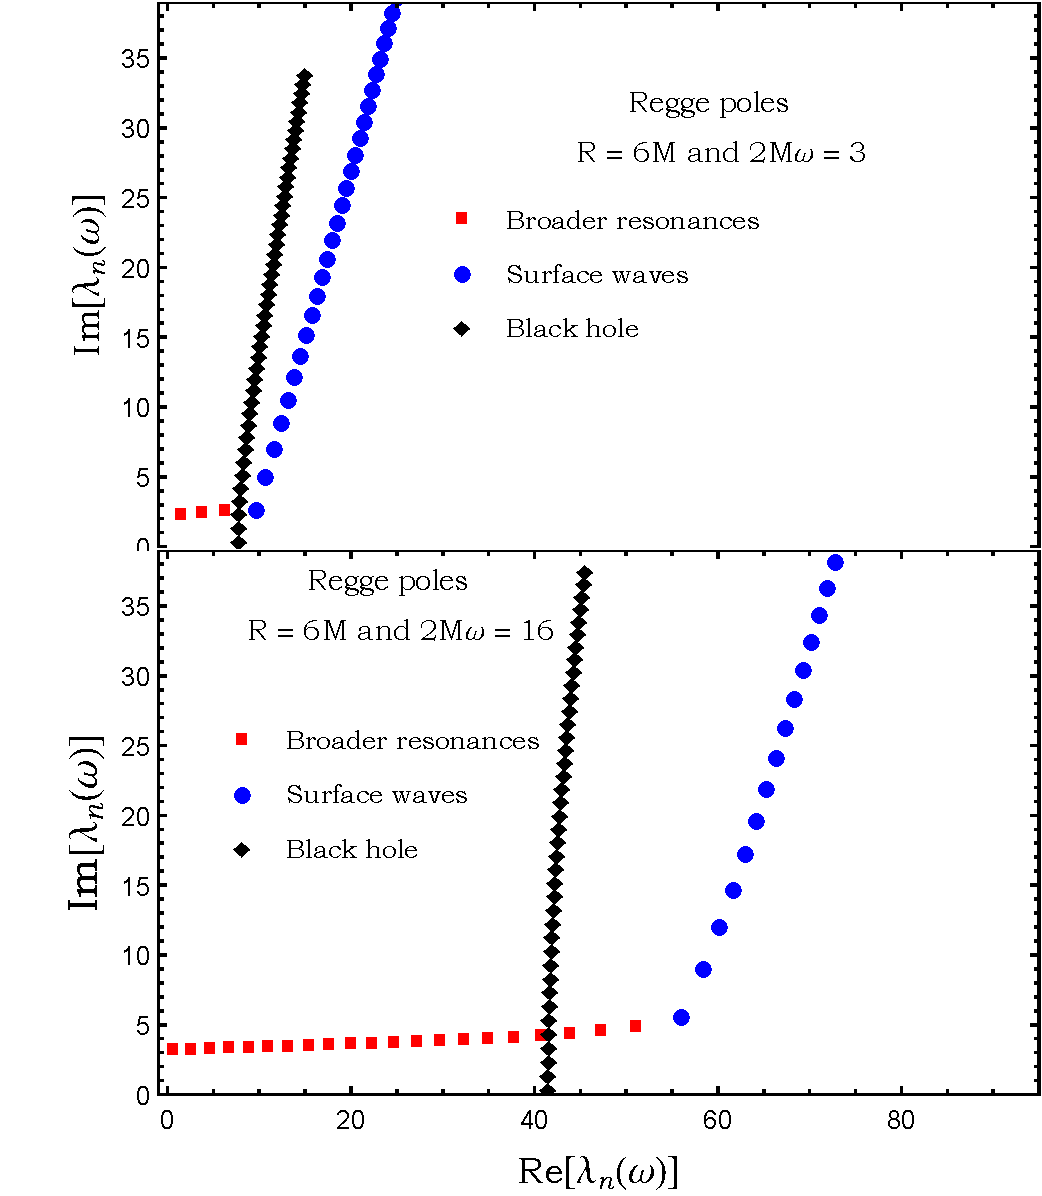
\includegraphics[scale=0.50]{RP_R_6_2Mw_3_16}
\caption{\label{RP_approx_2Mw_3_6_s_1} The Regge poles $\lambda_n(\omega)$ for the scalar field. We assume $2M =1$}
\end{figure}


 \begin{figure}[htb]
\centering
 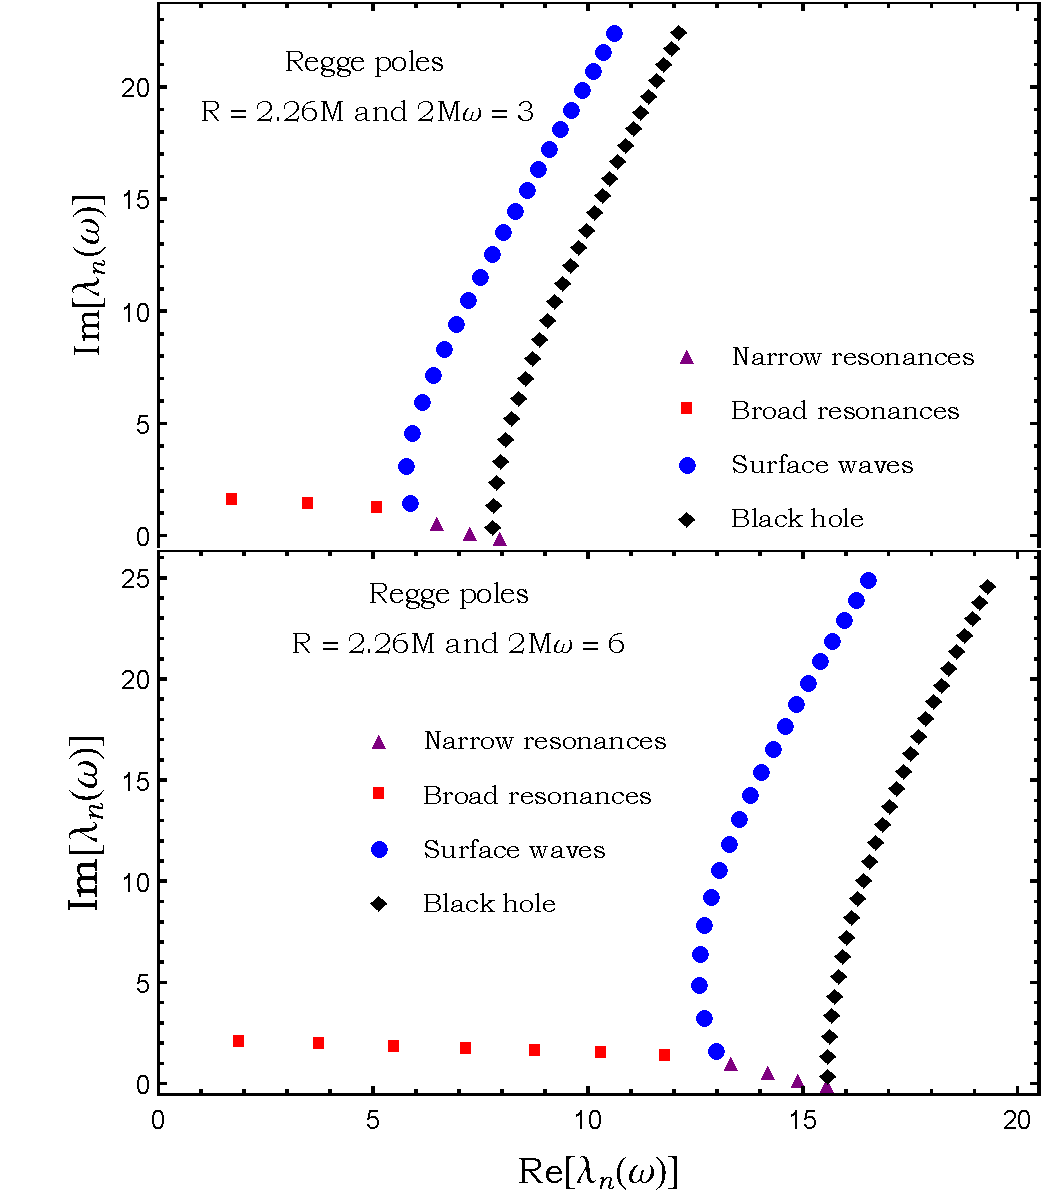
\includegraphics[scale=0.50]{RP_R_2_dot_26_2Mw_3_6}
\caption{\label{RP_approx_2Mw_3_6_s_1} The Regge poles $\lambda_n(\omega)$ for the scalar field. We assume $2M =1$}
\end{figure}


\begin{figure*}%[h!]
 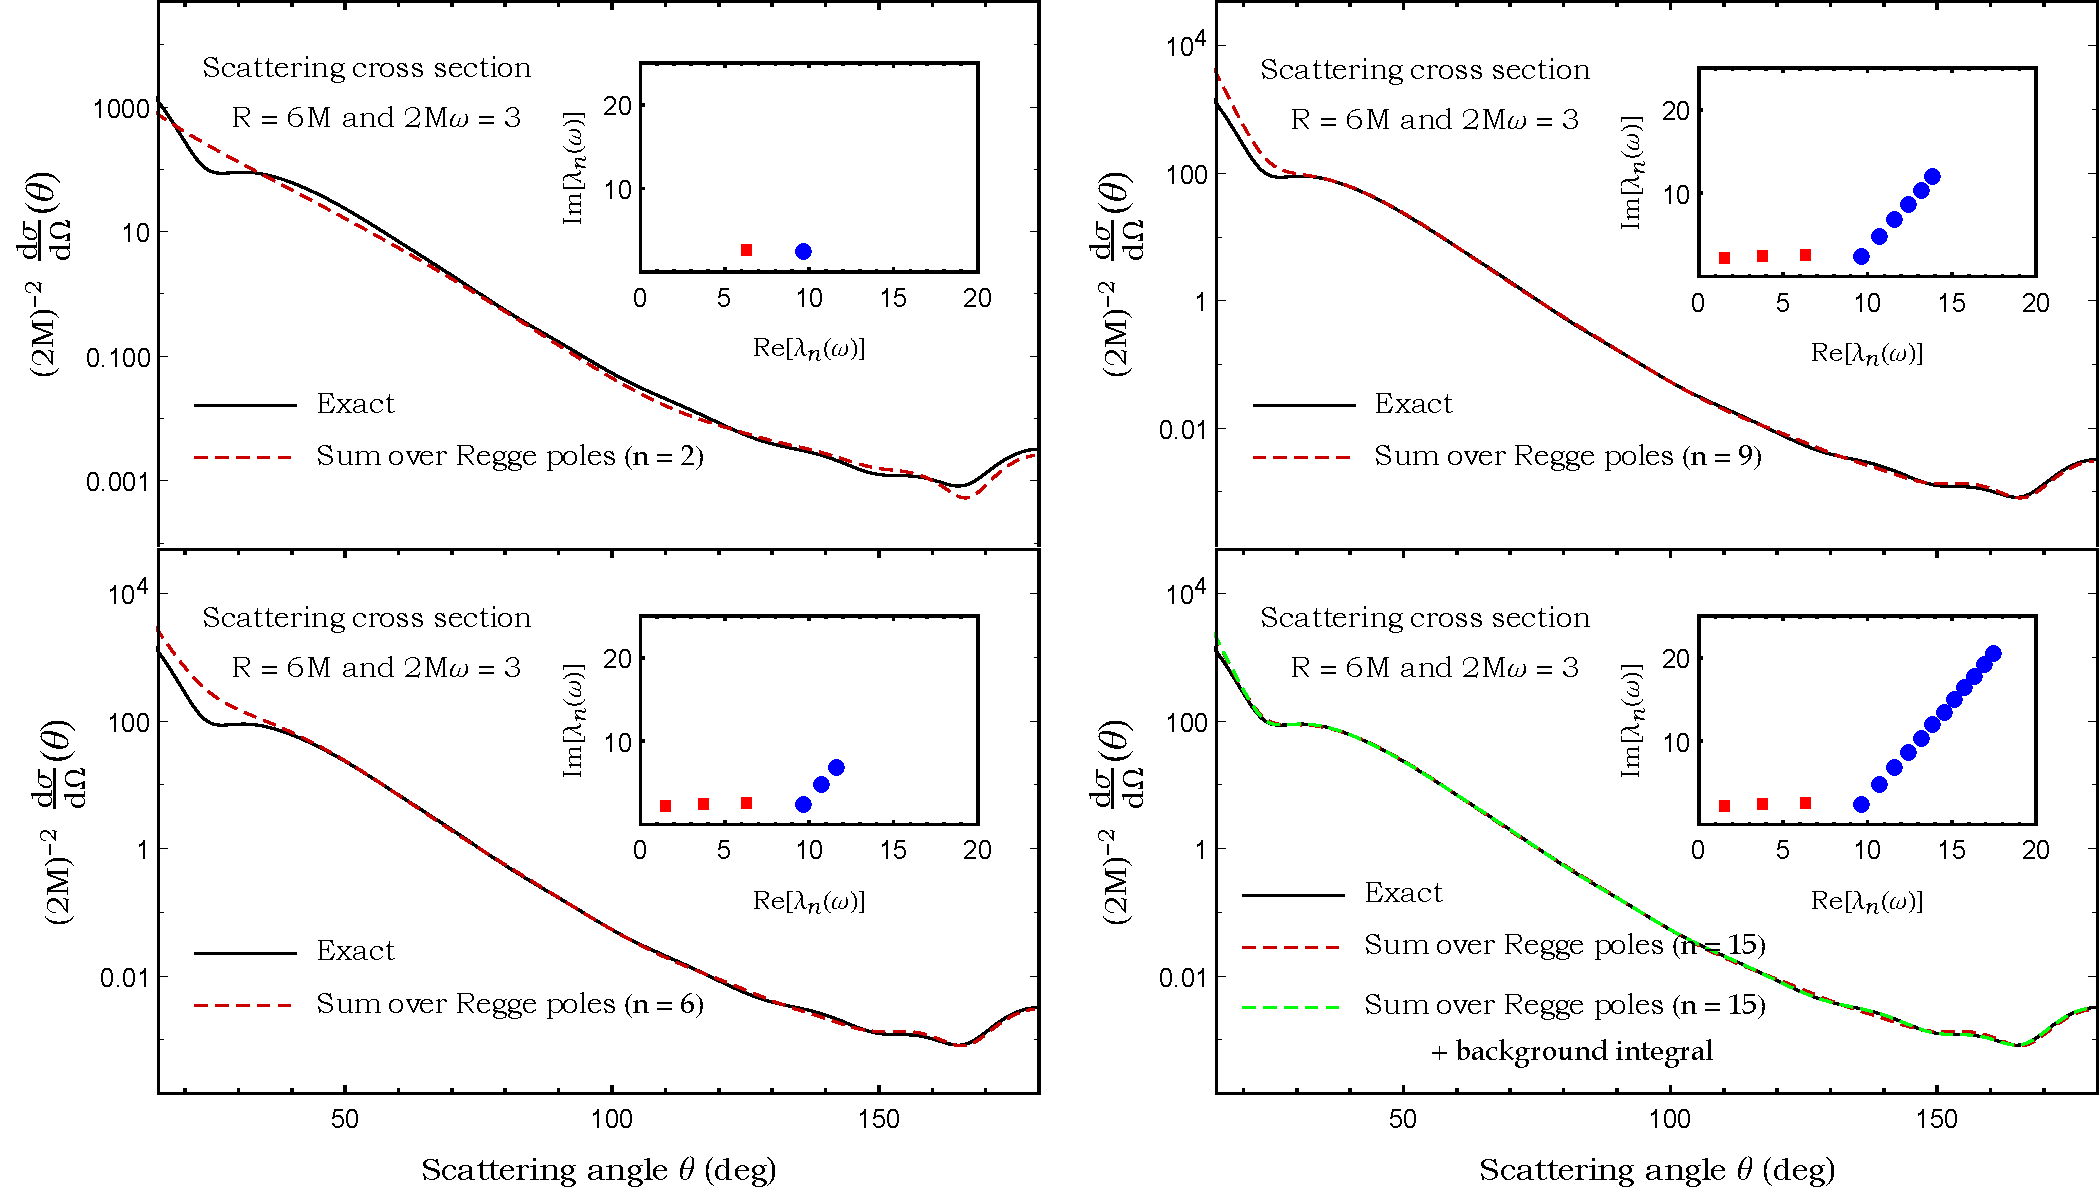
\includegraphics[scale=0.50]{Scattering_Cross_Section_R_6_2Mw_3}
\caption{\label{S_0_2Mw_01_Exact_vs_CAM} The scalar cross section of a compact bodies for $2M\omega=3$ and $R=6M$, its Regge pole approximation and the background integral contribution.}
\end{figure*}

\begin{figure*}%[h!]
 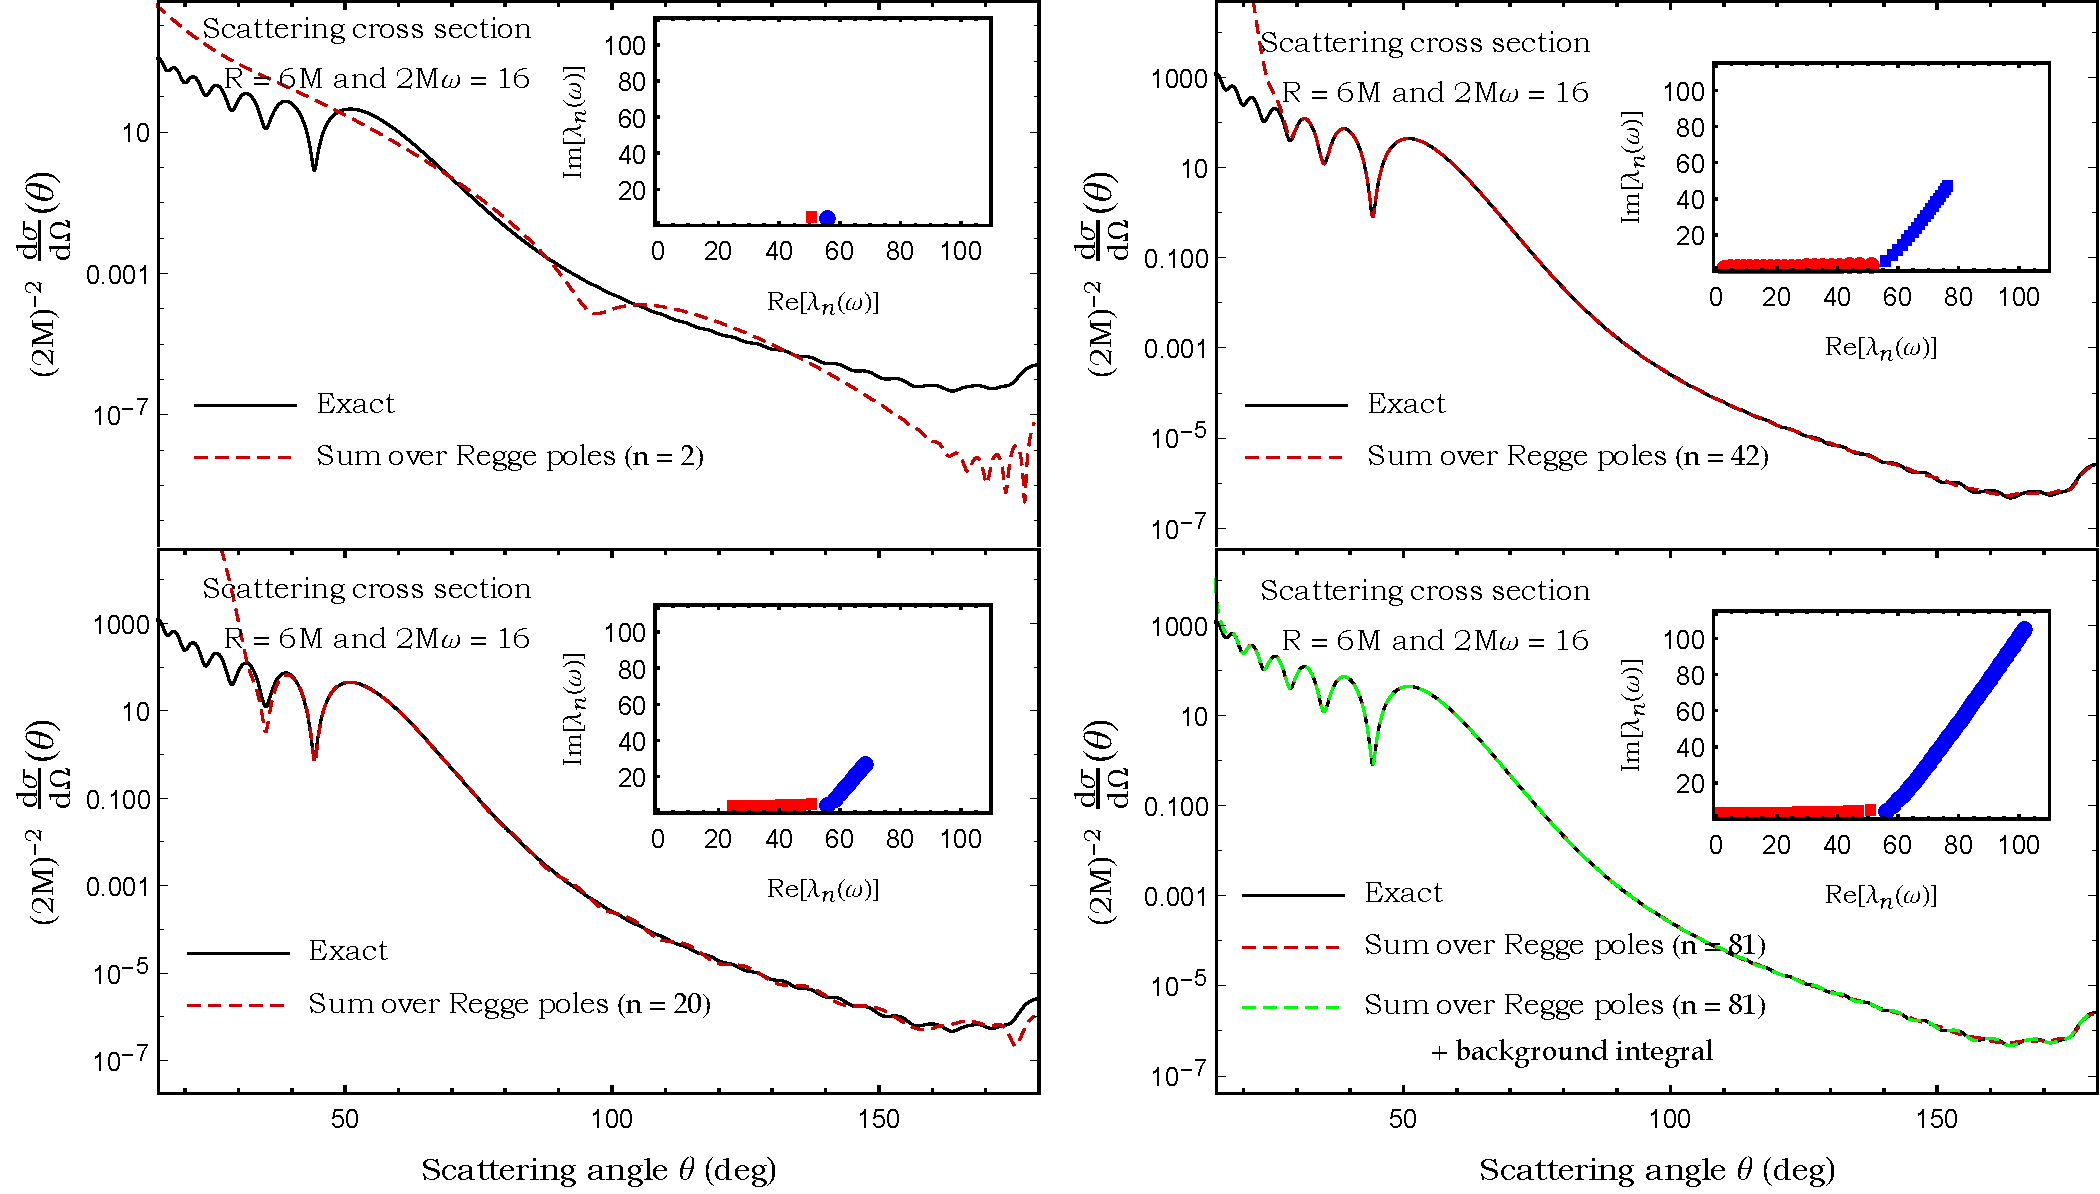
\includegraphics[scale=0.50]{Scattering_Cross_Section_R_6_2Mw_16}
\caption{\label{S_0_2Mw_01_Exact_vs_CAM} The scalar cross section of a compact bodies for $2M\omega=16$ and $R=6M$, its Regge pole approximation and the background integral contribution.}
\end{figure*}

\begin{figure*}%[h!]
\centering
 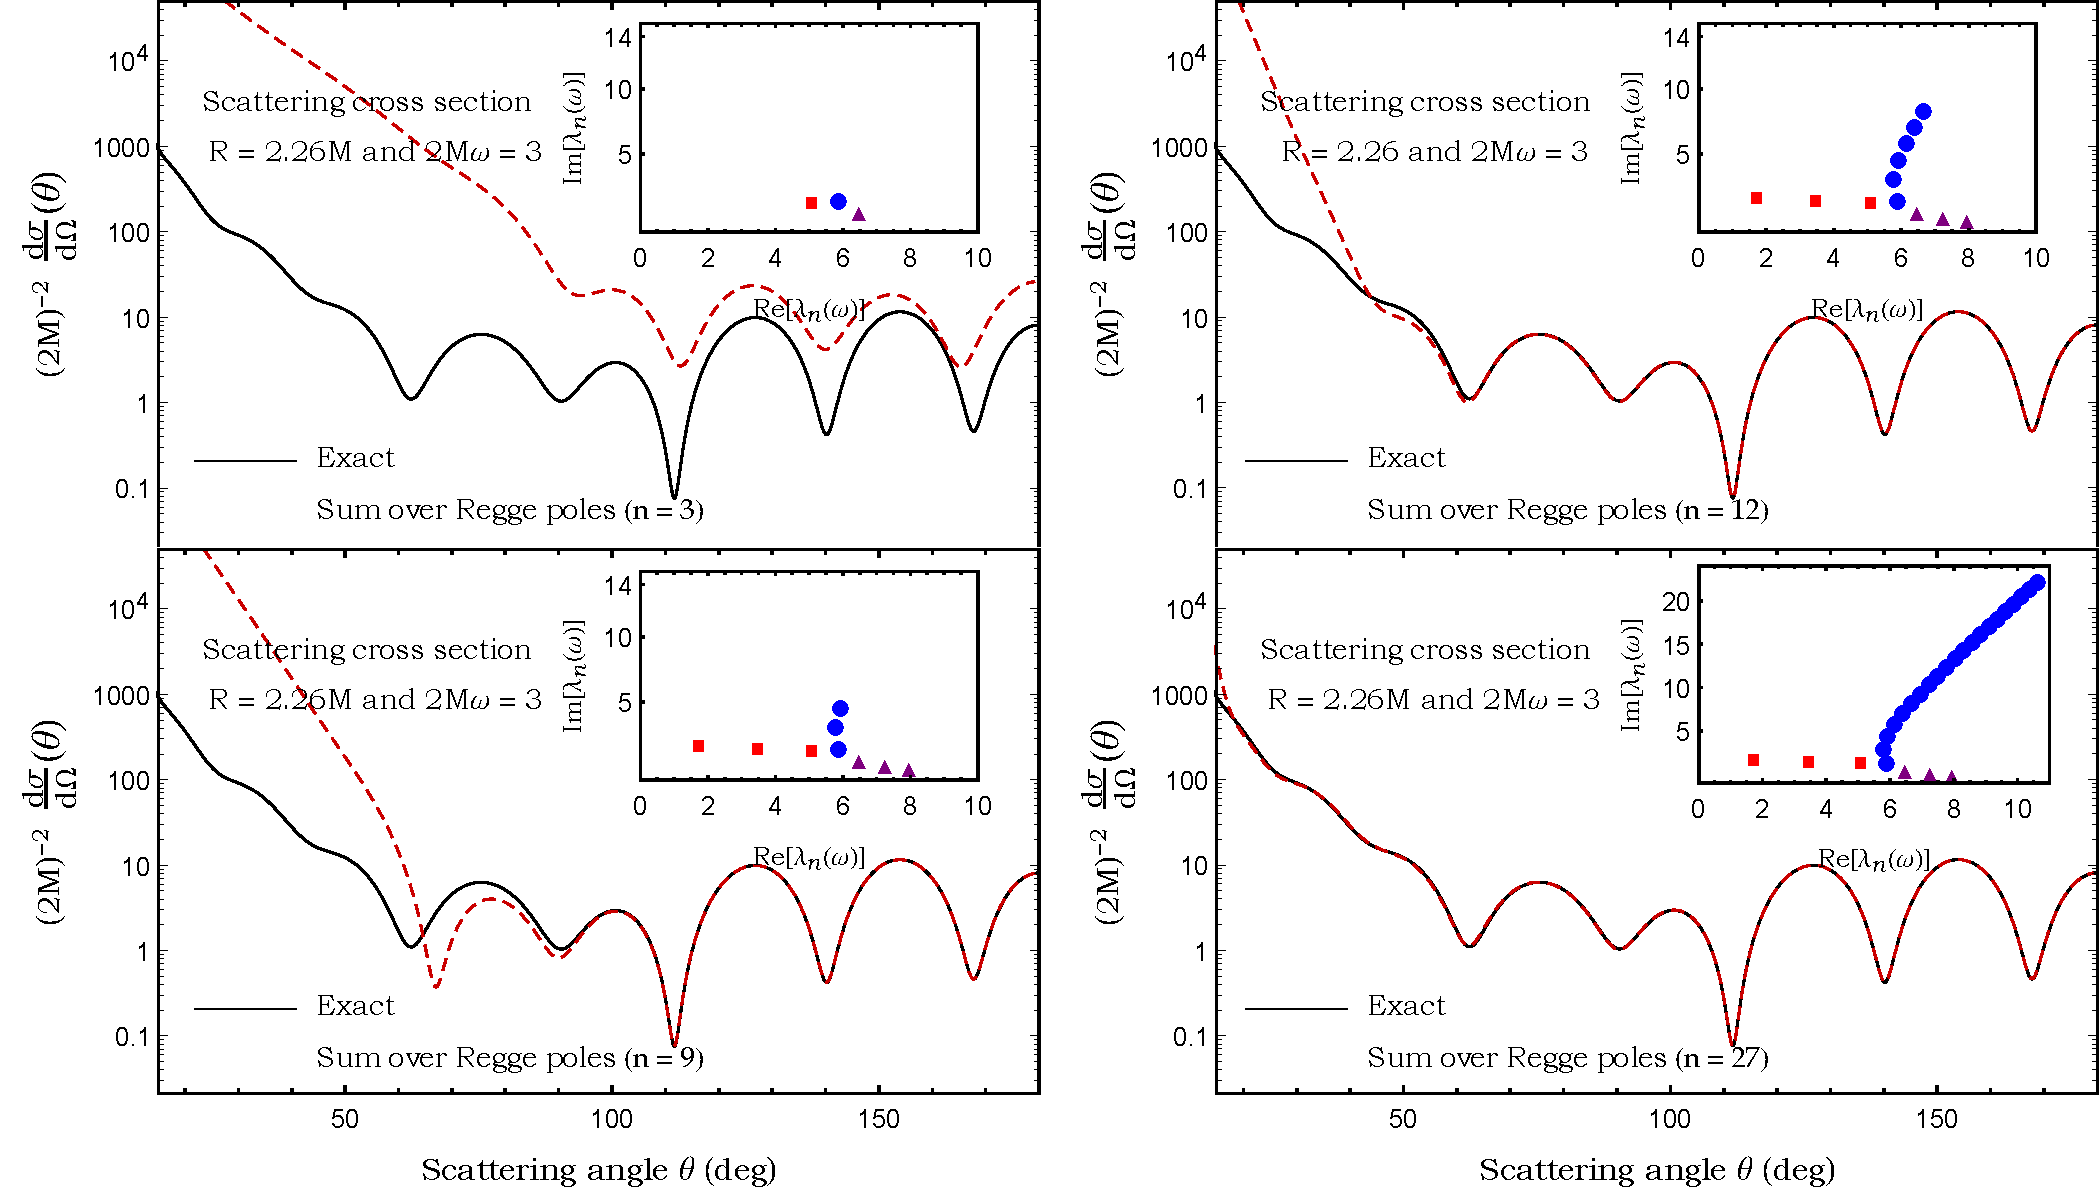
\includegraphics[scale=0.50]{Scattering_Cross_Section_R_2-dot-26_2Mw_3}
\caption{\label{S_0_2Mw_06_Exact_vs_CAM} The scalar cross section of a very compact bodies for $2M\omega=3$ and $R=2.26M$ and its Regge pole approximation.}
\end{figure*}


\begin{figure*}%[h!]
\centering
 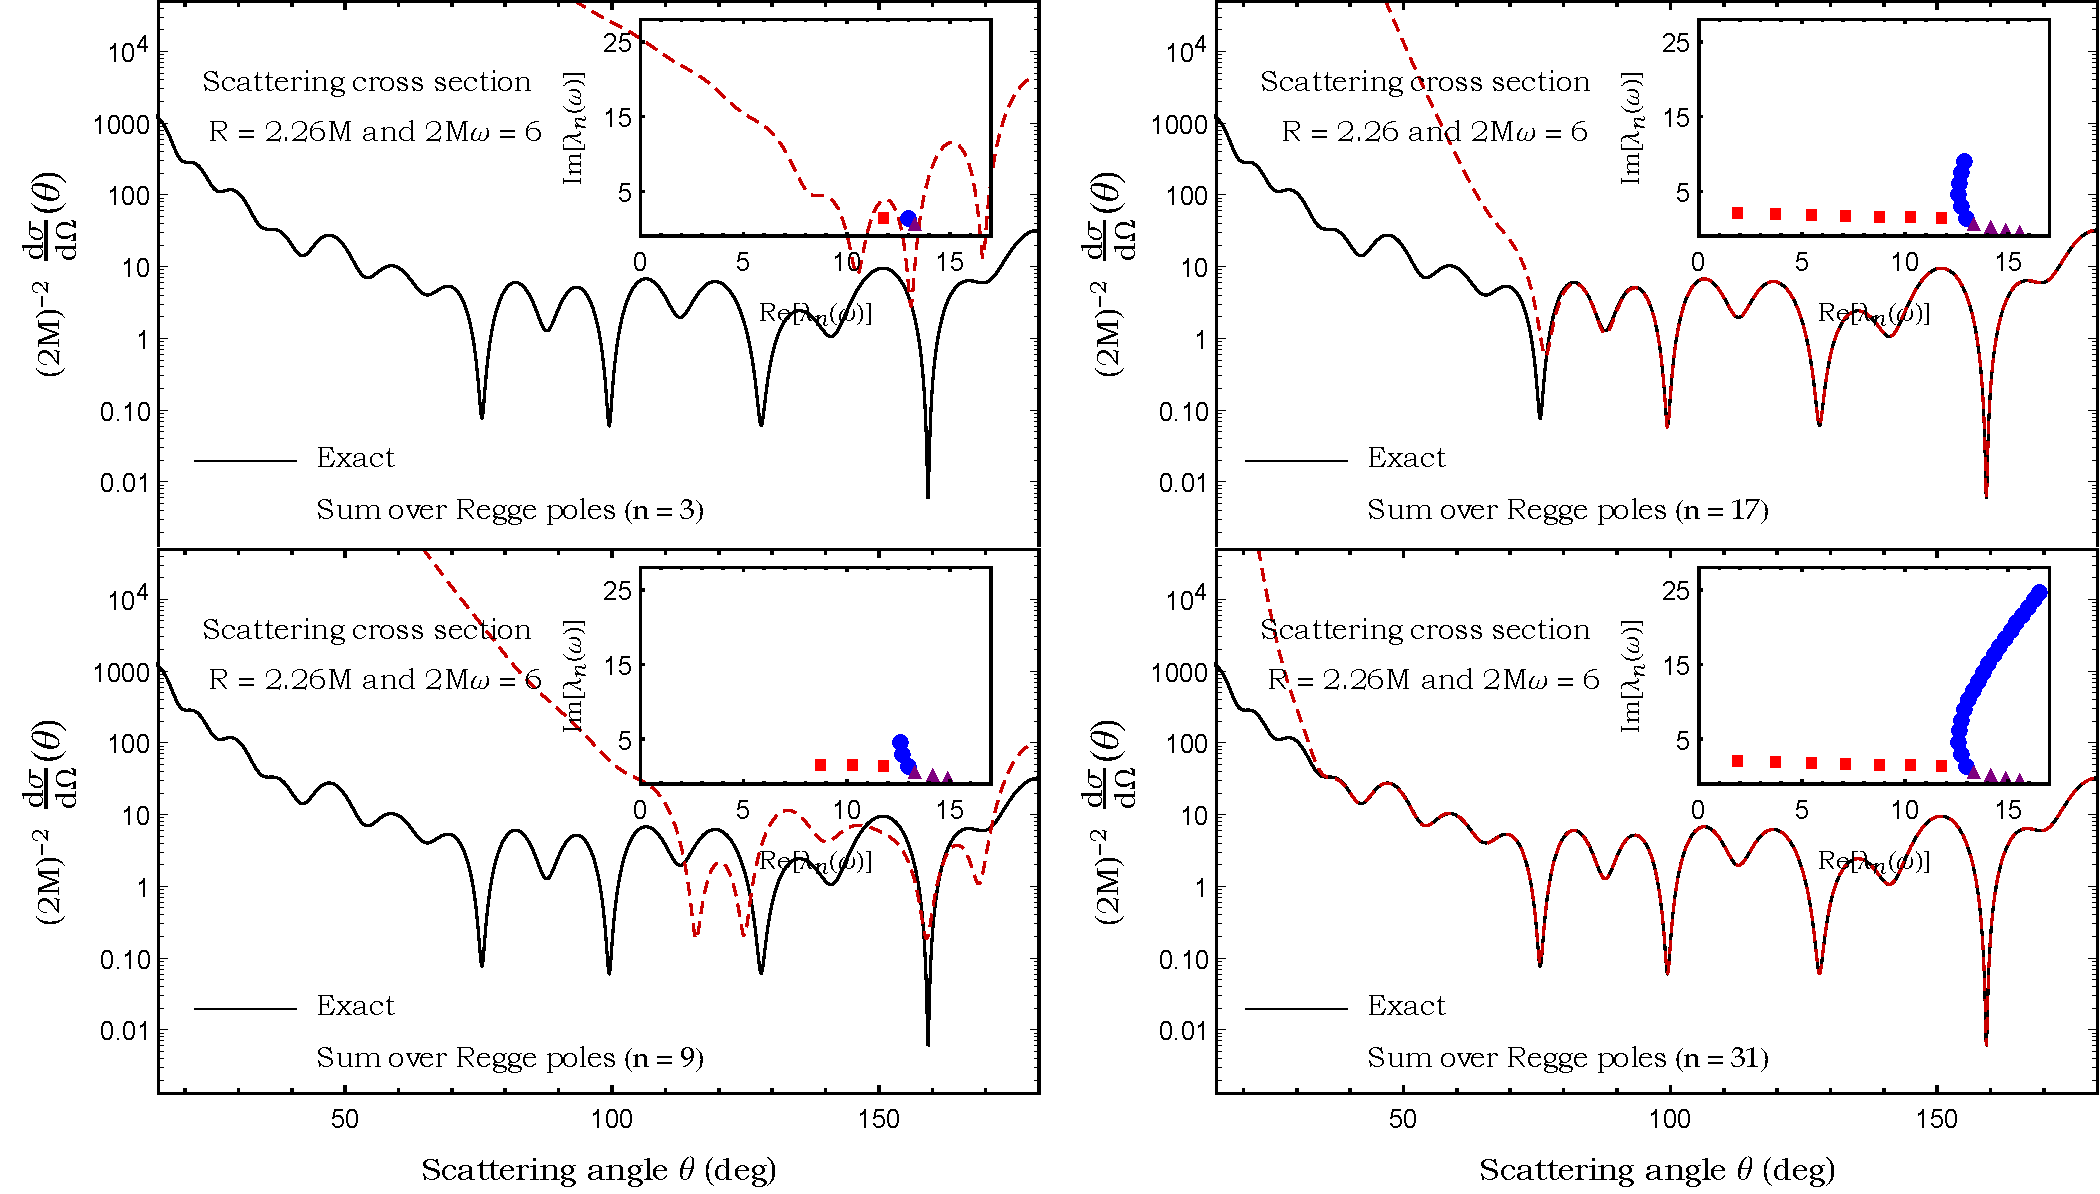
\includegraphics[scale=0.50]{Scattering_Cross_Section_R_2-dot-26_2Mw_6}
\caption{\label{S_0_2Mw_06_Exact_vs_CAM} The scalar cross section of a very compact bodies for $2M\omega=6$ and $R=2.26M$ and its Regge pole approximation.}
\end{figure*}


\begin{figure}%[h!]
\centering
 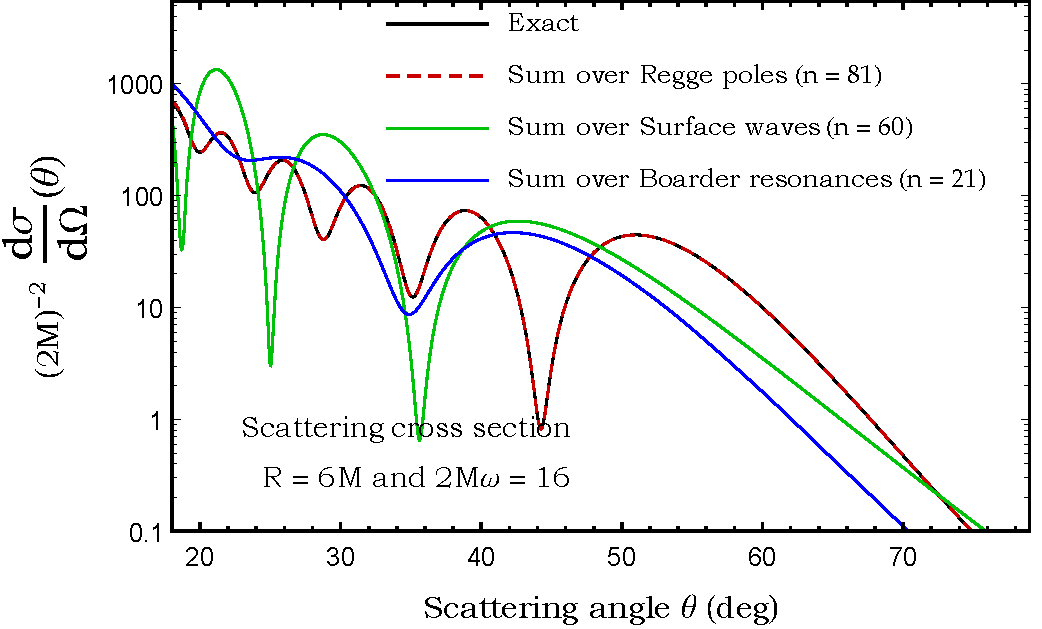
\includegraphics[scale=0.50]{Rainbow_Cross_Section_R_6_2Mw_16}
\caption{\label{S_0_2Mw_06_Exact_vs_CAM} Rainbow scattering for compact bodies for $2M\omega=16$ and $R=6M$, its Regge pole approximation and different contributions of the sum over Regge poles.}
\end{figure}


\begin{figure}%[h!]
\centering
 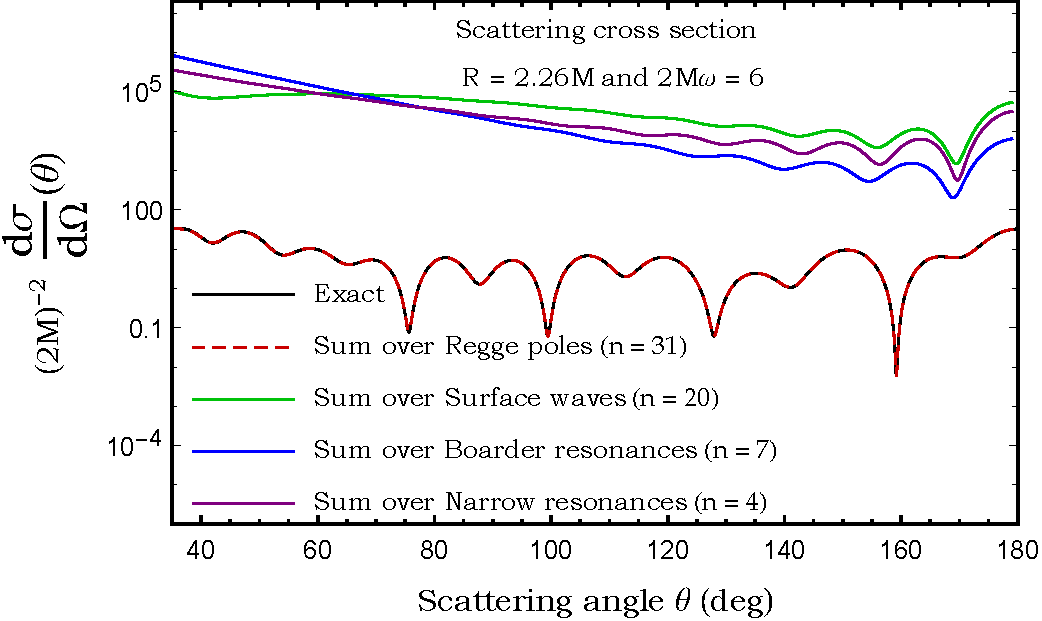
\includegraphics[scale=0.50]{Diff_Contribution_Cross_Section_R_2-dot-26_2Mw_6}
\caption{\label{S_0_2Mw_06_Exact_vs_CAM} Rainbow scattering for compact bodies for $2M\omega=16$ and $R=2.26M$, its Regge pole approximation and different contributions of the sum over Regge poles.}
\end{figure}


\begingroup
\squeezetable
\begin{table*}[htp]
\begin{threeparttable}[htp]
%\captionsetup{font=small}
\caption{\label{tab:table2} The lowest Regge poles $\lambda_{n}(\omega)$ for the scalar field and the associated residues $r_{n}(\omega)$. The radius of the compact bodies is $R = 6M$ and we assume $2M=1$.}
\smallskip
\centering
\begin{ruledtabular}
\begin{tabular}{cccccc}
 $n$ & $\omega$  & $\lambda^{\text{(S-W)\tnote{1}}}_n(\omega)$ & $\lambda^{\text{(B-R)\tnote{2}}}_n(\omega)$ & $r^{\text{(S-W)}}_{n}(\omega)$ & $r^{\text{(B-R)}}_{n}(\omega)$
 \\ \hline
$1$  & $3$  & $ 9.64850+2.76784 i$  & $1.56219+2.33072 i$  & $-12.41483-0.10424 i$  & $ -0.184457+0.480330 i$    \\
     & $16$  & $56.00945+5.71038 i$  & $ 0.62529+3.27098 i$  & $-447.5395+25.2912 i$  & $-0.322061-0.088002 i $  \\

$2$  & $3$  & $ 10.71986+5.16209 i $  & $3.81484+2.48159 i$  & $13.8486+24.3824 i$  & $0.290952+1.043116 i$    \\
     & $16$  & $ 58.442656+9.18793 i$ & $2.64868+3.31439 i$  & $5188.750-859.909 i$  & $ -0.381581-0.077583 i$    \\

$3$  & $3$  & $11.62296+7.17454 i$  & $ 6.35675+2.64104 i$  & $39.4189-12.3554 i$ & $2.83038-0.28686 i$    \\
     & $16$  & $60.20374+12.14965 i$  & $4.70011+3.35821 i$  & $-29331.71-18578.38 i$  & $-0.456423-0.021249 i$ \\

$4$  & $3$  & $ 12.4297+8.9960 i$  & $/$  & $ 13.2301-50.8802 i$ & $/$    \\
     & $16$  & $ 61.67700+14.84728 i $  & $6.78093+3.40257 i$  & $-15868.9+161199.9 i$  & $-0.528929+0.106794 i$ \\

$5$  & $3$  & $13.1734+10.6929 i$  & $/$  & $-33.7366-51.7404 i$ & $/$     \\
     & $16$  & $62.98626+17.37165 i$  & $8.89270+3.44762 i$  & $589920.5-79507.8 i$  & $-0.550038+0.330275 i$    \\

$6$  & $3$  & $13.8709+12.2989 i$  & $/$   & $-66.4436-20.7767 i$ & $/$    \\
     & $16$  & $ 64.18605+19.76911 i$  & $11.03720+3.49356 i$  & $-360464.-1.797518\times 10^6 i$  & $ -0.426365+0.639191 i$    \\

$7$  & $3$  & $14.5322+13.8342 i$  & $/$   & $-73.0825+21.9088 i$ & $/$     \\
     & $16$  & $65.30640+22.06743 i$  & $13.21653+3.54058 i$  & $-4.880638\times 10^6+646112. i$  & $-0.038292+0.926498 i$    \\

$8$  & $3$  & $15.1640+15.3122 i$  & $/$   & $-56.3641+59.6187 i$ & $/$     \\
     & $16$  & $66.36581+24.28491 i$  & $15.43310+3.5889 i$  & $-479098.+1.1836070\times 10^7 i$  & $0.652285+0.920876 i$    \\

$9$  & $3$  & $15.7709+16.7425 i$  & $/$   & $-25.0183+83.3731 i$ & $/$     \\
     & $16$  & $67.37659+26.43447 i$  & $17.6898+3.6390 i$  & $2.487209\times 10^7+7.72797\times 10^6 i$  & $1.363464+0.248276 i$    \\

$10$  & $3$  & $16.3565+18.1321 i$  & $/$   & $11.7631+90.6815 i$ & $/$     \\
     & $16$  & $68.34738+28.52564 i $  & $19.9900+3.6910 i$  & $3.163822\times 10^7-4.265475\times 10^7 i$  & $1.29469-1.13096 i$    \\
\end{tabular}
\end{ruledtabular}
\begin{tablenotes}
     \item[1] Surface waves
     \item[2] Broad resonances
   \end{tablenotes}
\end{threeparttable}
\end{table*}
\endgroup


\begingroup
\squeezetable
\begin{table*}[htp]
\begin{threeparttable}[htp]
%\captionsetup{font=small}
\caption{\label{tab:table2} The lowest Regge poles $\lambda_{n}(\omega)$ for the scalar field and the associated residues $r_{n}(\omega)$. The radius of the compact bodies is $R = 2.26M$ and we assume $2M=1$.}
\smallskip
\centering
\begin{ruledtabular}
\begin{tabular}{cccccccc}
 $n$ & $\omega$  & $\lambda^{\text{(S-W)\tnote{1}}}_n(\omega)$  & $\lambda^{\text{(B-R)\tnote{2}}}_n(\omega)$ & $\lambda^{\text{(N-R)\tnote{3}}}_n(\omega)$ & $r^{\text{(S-W)}}_{n}(\omega)$ & $r^{\text{(B-R)}}_{n}(\omega)$ & $r^{\text{(N-R)}}_{n}(\omega)$
 \\ \hline
$1$  & $3$  & $5.871590+1.553799 i$  & $1.73455+1.64951 i  $  & $ 6.48474+0.68765 i $  & $-179.7945+131.4187 i $ & $ -1.52081-2.30968 i$ & $-2.5672-15.3797 i $  \\
     & $6$  & $12.991923+1.754967 i $  & $ 1.89664+2.13696 i  $  & $ 13.34118+1.13496 i $  & $4356.193+647.790 i $ & $  -0.66176-1.31963 i$ & $  -390.218+379.906 i $  \\

$2$  & $3$  & $5.778805+3.228990 i  $  & $ 3.48084+1.45765 i$  & $  7.25606+0.24457 i$  & $428.6893-235.0321 i $ & $16.2123+5.2371 i $ & $ -0.272250-1.150335 i$  \\
     & $6$  & $12.705495+3.383881 i $  & $ 3.74238+2.01309 i $  & $14.18757+0.68182 i $  & $-35075.99-9772.94 i $ & $-2.93679+4.83548 i $ & $ -11.3519+34.5571 i $  \\

$3$  & $3$  & $ 5.924546+4.705899 i $  & $  5.10229+1.29099 i$  & $ 7.95763+0.01764 i$  & $-404.6185-390.8531 i$ & $ 70.4849+54.1888 i  $ & $ -0.0370202-0.0048174 i $  \\
     & $6$  & $12.596259+4.982661 i $  & $  5.49829+1.89576 i $  & $14.9017+0.2912 i $  & $82360.19+81990.53 i$ & $ 6.7872-16.9564 i$ & $0.27028+2.27905 i  $  \\

$4$  & $3$  & $ 6.144986+6.043188 i $  & $ /$  & $/ $  & $ -471.5443+314.3116 i  $ & $ /$ & $/ $  \\
     & $6$  & $ 12.614598+6.503749 i  $  & $ 7.17509+1.78279 i $  & $15.5621+0.0422 i  $  & $39281.5-229393.2 i  $ & $39.6176+33.5152 i  $ & $0.1011154+0.0020569 i $  \\

$5$  & $3$  & $6.398427+7.281723 i $  & $ /$  & $/ $  & $37.8777+546.8945 i $ & $ /$ & $/ $  \\
     & $6$  & $  12.71646+7.95208 i $  & $ 8.78112+1.67243 i  $  & $ /$  & $ -356055.5+34945.9 i$ & $ 2.1175+134.5962 i $ & $/ $  \\

$6$  & $3$  & $ 6.666837+8.447532 i $  & $/ $  & $ /$  & $418.7890+315.4209 i$ & $/ $ & $/ $  \\
     & $6$  & $ 12.87420+9.33552 i $  & $ 10.32300+1.56317 i$  & $/ $  & $45934.6+468157.5 i $ & $ 66.944+324.598 i$ & $/ $  \\

$7$  & $3$  & $ 6.941642+9.557619 i $  & $ /$  & $/ $  & $499.2703-37.6476 i $ & $ /$ & $ /$  \\
     & $6$  & $13.06993+10.66226 i $  & $ 11.80630+1.45720 i  $  & $ /$  & $558619.4+61956.5 i $ & $ 833.855+78.332 i $ & $/ $  \\

$8$  & $3$  & $7.218463+10.623548 i $  & $ /$  & $/ $  & $ 367.2578-307.7533 i  $ & $ /$ & $/ $  \\
     & $6$  & $13.29184+11.93979 i $  & $/ $  & $/ $  & $ 293571.8-559756.8 i $ & $/ $ & $/ $  \\

$9$  & $3$  & $ 7.494953+11.653498 i $  & $/ $  & $/ $  & $147.3038-435.8160 i  $ & $ /$ & $/ $  \\
     & $6$  & $ 13.53197+13.17461 i  $  & $/ $  & $/ $  & $ -376511.5-570254.0 i  $ & $/$ & $ /$  \\

$10$ & $3$  & $7.76982+12.65345 i $  & $/ $  & $/ $  & $-71.8294-437.3469 i  $ & $/ $ & $ /$  \\
     & $6$  & $ 13.78485+14.37216 i$  & $ /$  & $/ $  & $ -719306.1-20011.7 i $ & $ /$ & $/ $  \\

\end{tabular}
\end{ruledtabular}
\begin{tablenotes}
     \item[1] Surface waves
     \item[2] Broad resonances
     \item[3] Narrow  resonances
   \end{tablenotes}
\end{threeparttable}
\end{table*}
\endgroup

\section{WKB ?}
\label{SecIII}

The WKB approach developed by Zhang, Wu and Leung~\cite{Zhang:2011pq} to determine the axial \textit{w}-modes of a variety of stellar models can be adapted in order to obtain analytical approximations for the ``broad Regge poles'' for a scalar wave on a stellar background. The radial equation for axial gravitational perturbations is identical to Eq.~(\ref{H_Radial_equation}) but with the potential replaced by $V_{\ell} \rightarrow V_{\ell}^{\text{ax}}$ where \cite{Cardoso:2014sna}
\begin{eqnarray}\label{RW_Potentiel_axialGW}
V_{\ell}^{\text{ax}}(r) = f(r)\bigg[\frac{\ell(\ell+1)}{r^2}  - \dfrac{3 h(r)}{2r}\left(\dfrac{f'(r)}{f(r)}+\dfrac{h'(r)}{h(r)}\right) & \nonumber \\
	 + 8 \pi (p - \rho) & \bigg] .
\end{eqnarray}
%
We can expect then that Regge poles for axial gravitational perturbations are qualitatively the same as for scalar perturbations, and the methods discussed can be easily adapted to deal with either case.

\newcommand{\phiout}{\phi^{\text{out}}_{\omega, \lambda-1/2}}
\newcommand{\phireg}{\phi^{}_{\omega, \lambda-1/2}}

Regge poles and quasinormal modes for relativistic stellar models (of which \textit{w}-modes are a sub-category for gravitational perturbations) both satisfy the same wave equation and the same boundary conditions but with different interpretations for the angular momentum index and the frequency. Both types of pole satisfy the regularity condition at the origin~\eqref{bc_1_in} and the condition of a purely outgoing wave in the far field
%
\begin{equation}\label{bc_pole_inf}
\phiout (r) \scriptstyle{\underset{r_\ast \to +\infty}{\sim}}
\displaystyle{  A^{(+)}_{\lambda-1/2} (\omega) e^{+i\omega r_\ast}}.
\end{equation}
%
Thus, the Regge poles are solutions of Eq.~\eqref{H_Radial_equation} for which the  Wronskian of $\phireg$ and $\phiout$ vanishes (\textit{i.e.}, $A^{(-)}_{\lambda_n(\omega)-1/2} (\omega)=0$)
\begin{equation}\label{Wronskian}
  W[\phireg, \phiout ]= 0
\end{equation}
It has been shown that, the asymptotic expressions of $\phireg$ and $\phiout$ can be derived in certain regions, buy using the standard WKB approximation. In the high-frequency domain we have (see Refs \ldots)
\begin{equation}\label{Approx_origin}
  \phireg \underset{\omega \to \infty}{=} \omega r_* j_{\lambda-1/2} (\omega r_*) \quad\quad 0\leq r_*\leq R_*
\end{equation}
where $j_{\lambda-1/2}$ is the spherical Bessel function of the first kind and
\begin{equation}
\label{Approx_infinity}
\phiout  \scriptstyle{\underset{\omega \to \infty}{=}}
\left\{
\begin{aligned}
&e^{i\omega(r_*-R_*)}+\mathcal{R} e^{-i\omega (r_*-R_*)}& \scriptstyle{1/\omega\leq r_{*} < R_*,}\\
&\left(1+\mathcal{R}\right) e^{i\omega(r_*-R_*)}        & \scriptstyle{R_*\leq r_{*}<\infty.}
\end{aligned}
\right.
\end{equation}
Here
\begin{equation}\label{R_star}
  R_*=\int_{0}^{R}\, dr\,\frac{1}{\sqrt{f(r)h(r)}}
\end{equation}
and $\mathcal{R}$ is a reflection coefficient with the defintion given in Ref.~\cite{Berry_1982}.
Because the potential has a direct discontinuity at the surface of the compact body (see. Refs \cite{Zhang:2011pq,Berry_1982} for more details), we have for our model (\textit{i.e.}, compact body with a constant density)
\begin{equation}\label{R_reflection_1}
  \mathcal{R} = a \omega^{-2}
\end{equation}
with
\begin{eqnarray}
% \nonumber % Remove numbering (before each equation)
  a &=& -\left(\frac{i}{2}\right)^2 \lim_{\epsilon\to 0^{+}} \left[V_{\lambda-1/2}(r)\Bigg{|}_{r=R+\epsilon}-V_{\lambda-1/2}(r)\Bigg{|}_{r=R-\epsilon}\right] \nonumber\\
   &=& \frac{3M(R-2M)}{4 R^4}
\end{eqnarray}

%\begin{equation}\label{a_def}
%a= \frac{3M \left(R-2M\right)^2}{4 R^5}.
%\end{equation}
Now, by inserting the high frequency approximation for $j_{\lambda-1/2} (\omega r_*)$ into Eq.~\eqref{Approx_origin} \cite{nist},
\begin{equation}\label{Approx_origin_bis}
  \phi^{}_{\omega,\lambda-1/2} \underset{\omega \to \infty}{\approx} - \sin\left(\frac{\left(\lambda-1/2\right)\pi}{2}-\omega r_*\right)\quad\quad 0\leq r_*\leq R_*
\end{equation}
and Eq. \eqref{Approx_infinity} into the condition  \eqref{Wronskian}, we obtain
\begin{equation}\label{WKB_1}
   e^{ i\pi (\lambda-1/2)- 2 i \omega R_*}=-\mathcal{R}.
\end{equation}
%
We then solve Eq.~\eqref{WKB_1} and we obtain
\begin{equation}\label{lambda_Approx}
  \lambda_n \approx \frac{2 \omega R_*}{\pi}-\left(2n+\frac{1}{2}\right)+\frac{i}{\pi} \ln\left(\frac{1}{\mathcal{R}}\right)
\end{equation}
This corresponds to the series of Regge poles with spacing $|\Delta \lambda_n|\approx 2$ with the almost constant  imaginary part. Of course, they lie in the first quadrant of the CAM plan with a positive real part
%
\begin{equation}\label{Real_Part}
  \frac{2 \omega R_*}{\pi}-\left(2n+\frac{1}{2}\right)>0.
\end{equation}
%
The overtones are labelled by $n =1,2,\ldots$ and $n$ has an upper limit
%
\begin{equation}\label{Limit_Broad_RP}
n \leq \left\lfloor \frac{\omega R_*}{\pi} - \frac{1}{4}\right\rfloor.
\end{equation}
%
In other words, there is a finite number of the ``broad Regge poles''.

%\begin{equation}\label{lambda_Approx}
%  \lambda_n \approx \frac{2 \omega R_*}{\pi}+ 2 \left(n-\frac{1}{4}\right)+ 2\left\lfloor \ \frac{1}{2} - \frac{\text{Im}[2 i\omega R_*]}{2\pi} \right\rfloor - \frac{i}{\pi} \ln\left(\frac{a}{\omega^2}\right)
%\end{equation}


\begingroup
\squeezetable
\begin{table}[htp]
\caption{\label{tab:table3} The lowest Regge poles $\lambda_{n}(\omega)$ for the scalar field versus WBK results given by Eq.~\eqref{lambda_Approx}. The radius of the compact bodies is $R = 6M$ and we assume $2M=1$.}
\smallskip
\centering
\begin{ruledtabular}
\begin{tabular}{cccc}
 $n$ & $\omega$  & $\lambda^{\text{(B-R)}}_n(\omega)$ & $\lambda^{\text{(B-R, WKB)}}_n(\omega)$
 \\ \hline
$1$  & $3$  & $1.56219+2.33072 i$  & $1.592793+2.189767i$   \\
     & $16$ & $ 0.62529+3.27098 i$ & $0.661564+3.255453i $   \\

$2$  & $3$  & $3.81484+2.48159 i$  & $3.592793+2.189767i $    \\
     & $16$ & $2.64868+3.31439 i$  & $2.661564+3.255453i $    \\

$3$  & $3$  & $6.35675+2.64104 i$ & $5.592793+2.189767i $    \\
     & $16$ & $4.70011+3.35821 i$  & $4.661564+3.255453i $    \\

$4$  & $3$  & $/$  & $ / $   \\
     & $16$ & $6.78093+3.40257 i$  & $6.661564+3.255453i $  \\

$5$  & $3$  & $/$  & $/$     \\
     & $16$ & $8.89270+3.44762 i$  & $8.661564+3.255453i $   \\

$6$  & $3$  & $/$  & $/$    \\
     & $16$ & $11.03720+3.49356 i$ & $10.661564+3.255453i $ \\

$7$  & $3$  & $/$ & $/$     \\
     & $16$ & $13.21653+3.54058 i$  & $12.661564+3.255453i$ \\

$8$  & $3$ & $/$   & $/$     \\
     & $16$ & $15.4331+3.5889 i$  & $14.661564+3.255453i $  \\

$9$  & $3$ & $/$   & $/$   \\
     & $16$ & $17.6898+3.6390 i$  & $16.661564+3.384517i $   \\

$10$  & $3$  & $/$  & $/$   \\
     & $16$  & $19.9900+3.6910 i$  & $18.661564+3.255453i $  \\
\end{tabular}
\end{ruledtabular}
\end{table}
\endgroup


\section{Classification of quasinormal modes}

The study of stellar quasinormal modes began with a general relativistic extension of the Newtonian treatment of fluid pulsations of stars. Newly formed neutron stars, the remnants of supernovae collapse, are predicted to pulsate with a large initial energy \cite{thorne1967non}. It was and still is of interest to study how these pulsations lose energy in the form of gravitational waves. Recently, the gravitational waves from a neutron star merger were detected... In particular the emitted radiation should cary a signature of the modes of oscillation allowed inside the star. These fluid modes can be classified in analogy to their real Newtonian counterparts, with an additional damping time due to emission of GWs. Later, Kokkotas and Schutz showed that an additional family of modes existed \cite{Kokkotas:1986gd,Kokkotas:1992ka}, dubbed $\omega$-modes. These modes are characterised by a negligible excitation of fluid motion (and in the axial sector no fluid motion). They're highly damped and correspond to excitations of the dynamical perturbed space-time. For an excellent review of (gravitational) quasinormal modes in relativistic stars and black holes see \cite{Kokkotas:1999bd}.

We consider the massless scalar field which only couples to the body via gravitation. The scalar modes obey an equation of motion very similar to the axial gravitational wave sector. Accordingly, a similar spectrum for scalar modes can be expected (with no fluid excitation). Whilst these are arguably of less astrophysical interest, they are nonetheless a good model for axial GWs and allow us to make a first step towards a CAM approach for perturbed relativistic stars. We will classify the scalar $\omega$-modes as the axial GW modes have been, we have

	\begin{enumerate}
		\item Curvature modes: These modes exist for all relativistic stars. They are rapidly damped, and the damping is larger for less compact bodies.
		\item Trapped modes: These are the scalar analogue of the axial trapped modes considered by Chandrasekhar and Ferrari \cite{Chandrasekhar449}. They exist for bodies with $R/M < 3$. These models have an effective radial potential with a local minimum somewhere inside the star, and local maximum at the photon sphere $r=3M$. The trapped modes are essentially the first few curvature modes with energy less than the potential barrier. There are a finite number of them, and the number increases with the depth of the potential well.
		\item Interface modes: also known as $\omega_{\text{II}}$-modes, these were discovered by Leins \textit{et al.} \cite{Leins:1993zz}. They used a generalisation of Leaver's continued fraction  method as well as a `Wronskain method' that allowed them to accurately compute these modes which are characterised by very rapid damping (large imaginary part). This second branch of modes is the most similar to the Schwarzschild black hole quasinormal modes. We have taken their continued fraction method one step further (see section...) in order to be confident with our results.
	\end{enumerate}


\acknowledgments
M. O. E. H. wish to thank Antoine Folacci for various discussions concerning this work. T.S.~acknowledges financial support from EPSRC. S.R.D.~acknowledges financial support from the European Union's Horizon 2020 research and innovation programme under the H2020-MSCA-RISE-2017 Grant No.~FunFiCO-777740, and from the Science and Technology Facilities Council (STFC) under Grant No.~ST/P000800/1.



\bibliography{rainbowCAM}
%\bibliographystyle{apsrev4-1}

\end{document}
